\chapter{Podstawy teoretyczne}

\section{Rozpoznawanie emocji}

Rozpoznawanie emocji w dialogach koncentruje się na wydobyciu emocji przekazanej w rozmowie pomiędzy co najmniej dwoma rozmówcami. Problem ten stawia bardzo dużo wyzwań, takich jak obecność sarkazmu w rozmowie, przesunięcie emocji do kolejnych wypowiedzi tego samego rozmówcy oraz uchwycenie szerszego kontekstu pomiędzy wypowiedziami różnych osób. Dużym plusem w tej dziedzinie jest bardzo dobra dostępność do danych, które pochodzą z platform społecznościowych takich jak Facebook, Youtube, Reddit, Twitter \cite{poria2019emotion}. Poprzez łatwy dostęp do danych rozpoznawanie emocji w rozmowie staje się coraz bardziej popularne, a trudność tego problemu stwarza coraz to bardziej odległe granice co sprowadza się do wysokiego zainteresowania tą dziedziną przetwarzania języka naturalnego (ang. \textit{natural language processing - NLP}).

\section{Modele emocji}

Aby dobrze zrozumieć postawiony problem niezbędne będzie określenie czym są emocje. Wszyscy ludzie posiadają wrodzony zestaw podstawowych emocji, które można rozpoznać za pomocą gestów, czynów lub wypowiadanych słów. Możemy wyróżnić dyskretne emocje, aby móc odróżnić je od siebie.

\subsection{Model emocji Ekmana}

Istnieje kilka definicji różnych modeli emocji, jednym z nich jest model zaproponowany przez Paula Ekmana \cite{ekman1993facial}. Paul wraz ze współpracownikami stwierdzili, że istnieje sześć podstawowych emocji: gniew, obrzydzenie, strach, szczęście, smutek i zaskoczenie, a z każdą z tych emocji związane są jakieś cechy. Dzięki temu można wyrazić emocje w różnym stopniu a każda z nich jest zdefiniowana jako dyskretna kategoria, co pozwala na dość łatwą klasyfikację konkretnej emocji.

\subsection{Model emocji Plutchika}

Kolejną definicję modelu emocji przedstawił Robert Plutchik, który podzielił emocje na osiem podstawowych typów, z których każdy ma drobniejsze podtypy pokrewne \cite{plutchik1982psychoevolutionary}, zaprezentowane na rysunku \ref{rys:plutchik_wheel} za pomocą koła emocji. Prezentuje on emocje jako koncentryczne kręgi, gdzie wewnętrzne części odpowiadają za podstawowe emocje a te zewnętrzne za bardziej złożone. Model ten jest dyskretny, lecz widać w nim pewne zależności i podobieństwa pomiędzy sąsiadującymi częściami koła emocji. Budowa ta wynika ze złożoności emocji i możliwości wyrażania ich intensywności.

\begin{figure}[t]
\centering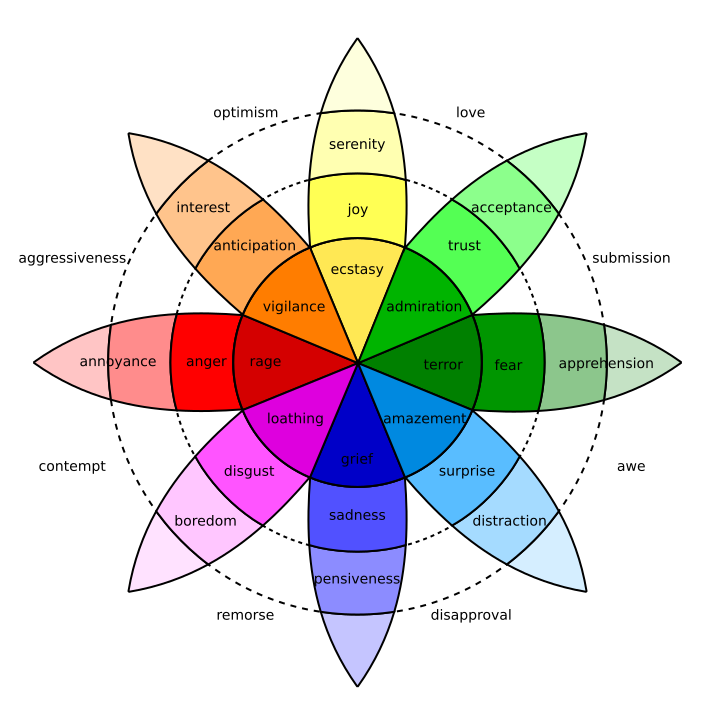
\includegraphics[width=10cm]{figures/plutchik-wheel.png}
\fcmfcaption{Koło emocji Plutchika \cite{plutchik1982psychoevolutionary}.}\label{rys:plutchik_wheel}
\end{figure}

\subsection{Porównanie modeli emocji}

Podsumowując wymienione modele emocji możemy wydzielić dwa główne typy: kategoryczne oraz wymiarowe. Modele wymiarowe mapują emocję w sposób ciągły na wektory. Modele kategoryczne klasyfikują emocję do konkretnej emocji dyskretnej, np. jednej z wybranego modelu emocji Ekmana lub Plutchika. Modele kategoryczne mają pewne wady. Jedną z nich jest brak możliwości opisania innych emocji oraz utrudnione opisywanie emocji złożonej z kilku różnych podtypów zdefiniowanych w dyskretnym modelu. Drugą wadą jest brak możliwości porównywania emocji, co umożliwiłby model wymiarowy, za pomocą porównywania dwóch wektorów. Wybór odpowiedniego modelu emocji nie jest łatwy, a jednocześnie jest bardzo ważnym elementem do późniejszej klasyfikacji emocji. Decydując się na kategoryczny typ emocji, z jednej strony mamy prosty model Ekmana który nie jest w stanie zamodelować złożonych emocji. Z drugiej strony w modelu Plutchika może być bardzo trudno rozróżnić drobnoziarniste emocje od siebie. Wybór ten należy zatem dokonać mając na uwadze wielkość oraz jakość zbioru danych.

\section{Głębokie uczenie}

Bardzo ważnym elementem w rozpoznawaniu emocji jest możliwość zrozumienia danego przekazu w kontekście, od którego może zależeć rodzaj emocji. Szczególnie trudnym przypadkiem jest zrozumienie i zapamiętanie kontekstu w konwersacji, co jak pokazują autorzy artykułu na temat architektury głębokiego uczenia do rozpoznawania emocji w rozmowach tekstowych \cite{zhong2019knowledgeenriched}, może okazać się kluczowym czynnikiem skuteczności tych metod. Do uzyskania satysfakcjonujących wyników nie wystarczają tradycyjne metody uczenia maszynowego lub najbardziej podstawowe architektury sieci neuronowych \cite{kowsari2019text}. Niezbędne jest użycie sieci rekurencyjnych oraz różnych rozszerzeń pozwalających na zapamiętanie i zrozumienie kontekstu w tekście.

\subsection{Rekurencyjne sieci neuronowe}

Tradycyjne sieci neuronowe nie są w stanie podejmować decyzji na podstawie sekwencji zdarzeń, w tym przypadku kolejnych słów w zdaniu. Sieci rekurencyjne wykorzystują informacje zawarte w całej sekwencji za pomocą powiązania wyjścia z komórek do następnych obliczeń w tej samej komórce. Dodatkowo każda komórka może używać swojej pamięci wewnętrznej do przechowywania informacji o poprzednim wejściu. Sieci rekurencyjne bardzo dobrze radzą sobie w problemach przetwarzania tekstu, rozpoznawania mowy a także szeregów czasowych. Umożliwiają one zrozumienie kontekstu wypowiedzi na podstawie pozostałych słów znajdujących się w zdaniu.

\subsection{Sieci rekurencyjne LSTM}

Rozszerzeniem zastosowania rekurencyjnych sieci neuronowych jest zastosowanie bardziej złożonych komórek. Przykładem są komórki LSTM (ang. \textit{Long Short-Term Memory}), które w przeciwieństwie do standardowych komórek sieci neuronowych, posiadają połączenia zwrotne, umożliwiające zapamiętanie sąsiednich stanów w sieci. Dodatkowo są odporne na wygaszanie długotrwałych zależności w zdaniu. Jest to sytuacja w której znaczenie danego słowa zależy od słowa znajdującego się dużo wcześniej w zdaniu. Komórki LSTM złożone są z kilku modułów umożliwiających zapamiętanie długotrwałych zależności. Głównym elementem jest komórka pamięci, która utrzymuje swój stan w czasie. Dodatkowo występują jednostki bramki (ang. \textit{gates}), które decydują o tym jaką część informacji brać do obliczeń w obecnym kroku i regulują przepływ informacji płynących do oraz z komórek pamięci. Szczegóły budowy oraz porównanie do tradycyjnych komórek sieci rekurencyjnych (RNN) zaprezentowano na rysunku \ref{rys:rnn_vs_lstm}.

\begin{figure}[t]
\centering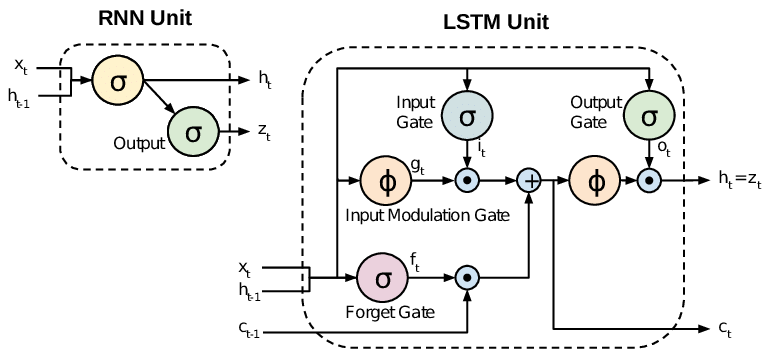
\includegraphics[width=10cm]{figures/rnn_vs_lstm.png}
\fcmfcaption{Porównanie komórek rekurencyjnych (RNN) z komórkami LSTM.}\label{rys:rnn_vs_lstm}
\end{figure}

\section{Transfer wiedzy lingwistycznej}

W przetwarzaniu języka naturalnego z użyciem głębokich sieci neuronowych coraz częściej używane są techniki transferu wiedzy (ang. \textit{transfer learning}) oraz adaptacji domenowej. Model języka jest kluczowym elementem do zastosowania powyższych technik. Umożliwia on przewidzenie kontekstu w jakim dane słowo znajduje się w zdaniu i na tej podstawie umożliwia odkryć jego prawdziwy sens. Jest uważany za bardzo istotny element w dziedzinie \textit{NLP}, który stanowi podstawę do wszelkich zastosowań przetwarzania języka naturalnego. Najważniejsze jego cechy to zrozumienie długofalowych zależności i hierarchicznej struktury tekstu, a największe zalety to otwarte i wolne zasoby do jego stworzenia. Jest tworzony za pomocą nienadzorowanego procesu uczenia, który potrzebuje tylko korpusu nieoznakowanego tekstu.

\subsection{Metoda ULMFIT}

Znakomitym przykładem użycia transferu wiedzy za pomocą wielokrotnego uczenia modelu języka jest metoda \textit{ULMFIT} \cite{howard2018universal} (ang. \textit{Universal Language Model Fine-tuning for Text Classification}, która może być zastosowana do każdego zadania w NLP. Zastosowane są w niej techniki, które są kluczowe dla dostrojenia modelu językowego. Używane są w niej 3 warstwy sieci neuronowej wykorzystującej komórki LSTM. Dodatkowo zastosowana jest technika przerywania (ang. \textit{dropout}) niwelująca problem przeuczania. Cały etap nauki w metodzie \textit{ULMFIT} składa się z 3 etapów zaprezentowanych na rysunku \ref{rys:ulmfit}. Na początku następuje szkolenie wstępne modelu językowego na dowolnym korpusie, następnie dostrojenie modelu językowego na zadaniu docelowym i na końcu dostrojenie klasyfikatora na zadaniu docelowym. Dzięki zastosowaniu tych technik możliwe jest wyuczenie wstępne modelu języka na dowolnych danych, (np. korpus Wikipedii) a następnie wykorzystanie tego wstępnie wyuczonego modelu na zadaniu docelowym. Na podobnej zasadzie działają dzisiejsze najbardziej wyrafinowane architektury głębokich sieci neuronowych w zastosowaniu przetwarzania języka naturalnego nazywane aktualnym stanem techniki (ang. \textit{state of the art}).

\begin{figure}[t]
\centering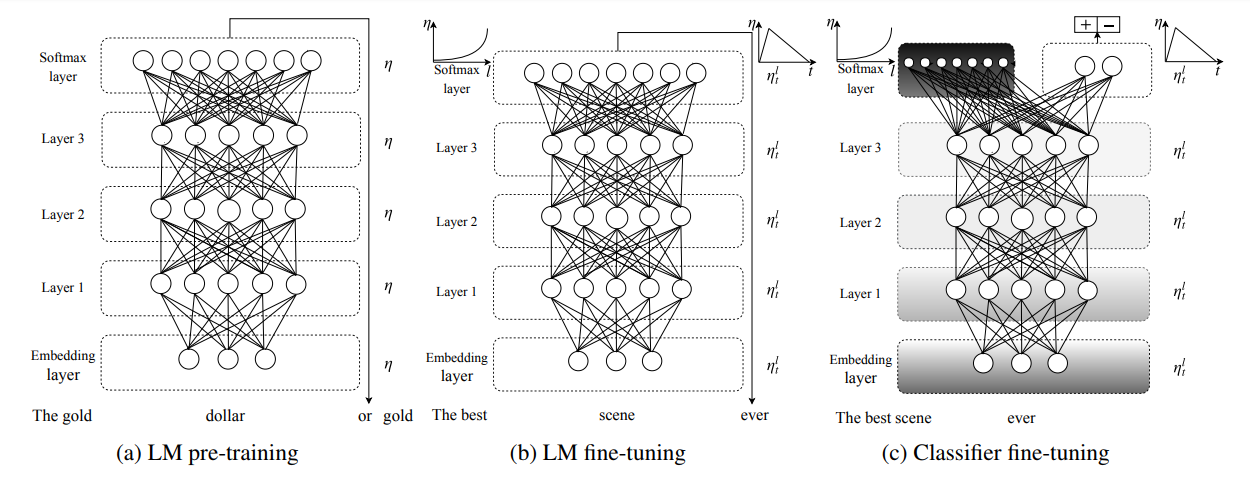
\includegraphics[width=\textwidth]{figures/ulmfit.png}
\fcmfcaption{3 etapy nauki modelu języka (ang. \textit{LM}) w metodzie ULMFIT \cite{howard2018universal}.}\label{rys:ulmfit}
\end{figure}

\subsection{Architektura transformera}

Transformer (ang. \textit{The Transformer}) \cite{vaswani2017attention} jest to model który wykorzystuje mechanizm uwagi, inaczej samoobserwacji (ang. \textit{self-attention}) do przyspieszenia procesu nauki. Główny jego cel to poprawa modelowania sekwencja do sekwencji (ang. \textit{Seq2Seq}) poprzez samoobserwację  i kodowanie pozycji (ang. \textit{positional encoding}). Składa się on z dwóch głównych komponentów zaprezentowanych na rysunku \ref{rys:attention_transformer}. Jest to część kodująca (po lewej stronie) oraz część dekodująca (po prawej stronie), które są ze sobą połączone.

Elementem kodującym jest stos koderów o tej samej strukturze. Pierwszą warstwą każdego kodera jest mechanizm samoobserwacji. Umożliwia to łączenie znaczenia danego słowa z innymi słowami w zdaniu, poprzez kodowanie danego słowa. Wyjście z warstwy samoobserwacji przekazywane jest do sieci neuronowej typu \textit{feed-forward}, która jest stosowana do każdej pozycji w zdaniu.

W części dekodującej także znajduje się stos dekoderów o tej samej liczności co koderów. Wszystkie z nich mają identyczną strukturę, podobną do struktury kodera. Dodatkowo pomiędzy warstwami występującymi w koderze znajduje się dodatkowa warstwa uwagi, która pomaga dekoderowi skupić się na odpowiednich częściach zdania wejściowego. 

Zdanie jest przetwarzane na reprezentację wektorową na wejściu pierwszego kodera. Maksymalna szerokość tego wektora to 512. Wektor ten, jako reprezentacja zdania wejściowego przechodzi przez każdą z dwóch warstw kodera. 

Najważniejszą częścią budowy tego modelu jest wspomniany wcześniej mechanizm samoobserwacji, który pozwala na tak dobre zrozumienie danych słów w kontekście całego zdania. Podczas gdy model przetwarza każde słowo, uwaga własna pozwala mu patrzeć na inne słowa w zdaniu w celu poszukiwania wskazówek, które mogły by pomóc w lepszym zakodowaniu tego słowa. Dzięki temu podobnie jak w rekurencyjnych sieciach neuronowych możliwe jest zrozumienie znaczenia danego słowa poprzez zapamiętanie znaczenia pozostałych słów w zdaniu. 

\begin{figure}[t]
\centering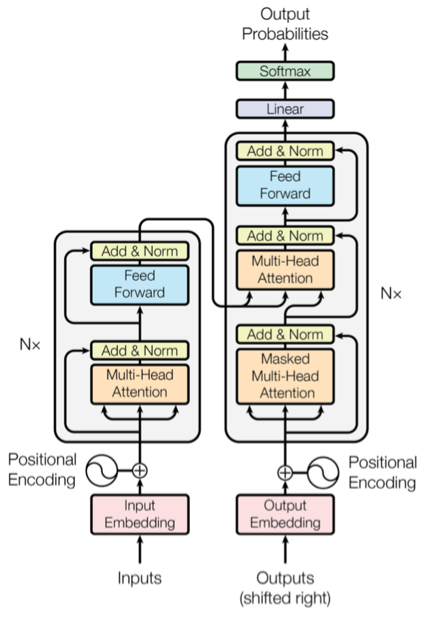
\includegraphics[width=6cm]{figures/attention_transformer.png}
\fcmfcaption{Architektura modelu transformera \cite{vaswani2017attention}.}\label{rys:attention_transformer}
\end{figure}

\subsection{BERT}

Rok 2018 był przełomowy dla modeli uczenia maszynowego przetwarzających tekst, a wydanie BERT (ang. \textit{Bidirectional Encoder Representations from
Transformers}) określane jest jako początek nowej ery w dziedzinie przetwarzania tekstu. Architektura ta jest niejako następcą metody ULMFIT oraz Transformera, gdyż główne jej założenia wywodzą się właśnie z tych metod. Wkrótce po wydaniu artykułu opisującego metodę \cite{devlin2018bert}, zespół z Google udostępnił także kod źródłowy modelu, który umożliwia użycie tej architektury w uproszczony sposób. 

Architektura tej metody składa się ze stosu koderów zaprezentowanych dla Transformera. Każdy z nich zawiera warstwę samoobserwacji oraz sieć neuronową typu \textit{feed-forward}. Dodatkowo używana jest metoda dwukierunkowej nauki, która umożliwia osiągnięcie jeszcze lepszego wyniku.

BERT opiera się na sposobie trenowania podobnym do przedstawionego w metodzie ULMFIT. Jest to częściowo nadzorowane uczenie na dużym zbiorze danych. Wykorzystane są metody pozwalające na efektywne wykorzytsanie tego, czego model uczy się podczas wstępnego treningu. Wprowadza on bowiem model językowy, który pozwala na efektywne użycie wiedzy lingwistycznej do zastosowania w problemach przetwarzania tekstu. Sam proces nauki tego modelu jest oparty o dwa zadania które umożliwiają obliczenie funkcji strat, są to problemy przewidywania następnego zdania oraz rozpoznanie ukrytego słowa w zdaniu.

Model BERT może być używany do wielu różnych zadań językowych, za pomocą drobnych modyfikacji jednej z ostatnich warstw. Bardzo dobrze sprawdza się w zadaniach rozpoznawania par zdań, rozpoznawania sentymentu, odpowiadanie na pytania czy tagowania zdań. Wszystkie te problemy przedstawione są na rysunku \ref{rys:bert_problems}.

\begin{figure}[t]
\centering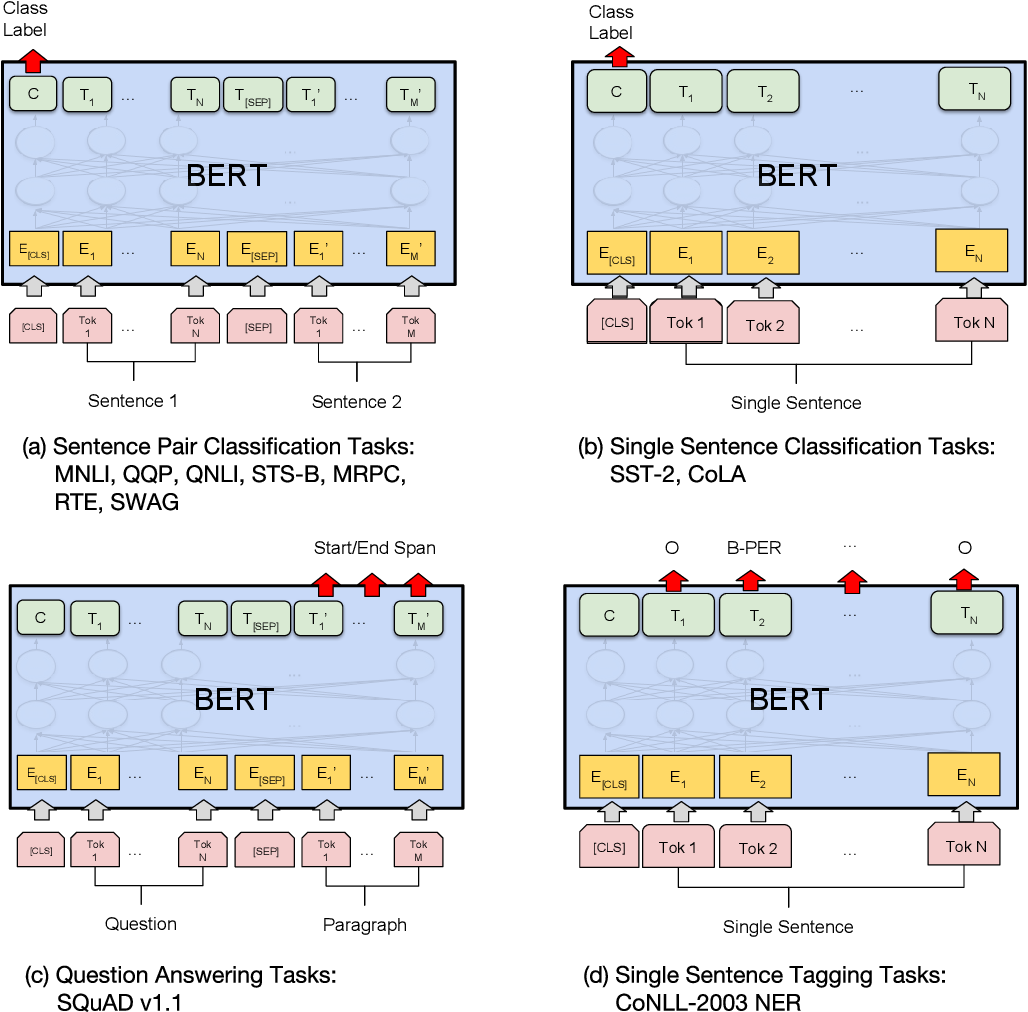
\includegraphics[width=12cm]{figures/bert_problems.png}
\fcmfcaption{Zastosowanie BERT do różnych problemów \cite{devlin2018bert}.}\label{rys:bert_problems}
\end{figure}